\chapter{序論}
\label{chap:introduction}
\section{背景}

% なぜこの研究が必要だったのか、しっかりした理屈を考えておく。
% 現状どういう問題があるのか
% どういう方法で解決を試みたのか
% 結果として上手く行ったのか、いかなかったのか

近年、スマートフォンなどのモバイルインターネット端末は爆発的に普及し、利用者の年代を問わず用いられるようになった。
生活の一部とも言える存在となったこれらの端末だが、私がこれらの端末を使用する中で不便だと感じる点がある。
それは取得したいと思う情報を思うように得られないという点である。スマートフォンを用いて情報を獲得する手法としてAndroid Widgetは普遍的に用いられている。
天気予報を見たければ天気予報のWidgetを画面に設置し、別の情報が必要であればまた別のWidgetを設置する。
設置してさえおけばユーザーが能動的に操作をしなくとも最新の情報を常に画面に表示してくれるので情報の獲得手法としては有能である。

しかし、Android Widgetは多くの問題点も抱えている。
まずAndroid端末の一つの画面に置くことの出来るWidgetの数は限られているため獲得できる情報の種類も限られてしまうという問題である。(図\ref{fig:old_widget})
しかもAndroid Widgetの性質上取得したい情報に付随して不要な情報までもが表示され、それによって画面スペースを埋められてしまうといったケースも存在する。
また、自分の取得したい情報に対応したWidgetが存在しない場合、自らWidgetを作成するしか無いといった問題もある。
現状ではAndroid Widgetの作成は技術的なハードルが高く問題の解決法としては現実的ではない。

そこで私はあらゆる情報に対応した汎用的なAndroid Widgetを作成することでこれらの状況を解決したいと考えた。

\begin{figure}[htbp]
  \begin{minipage}{\hsize}
    \begin{center}
      \fbox{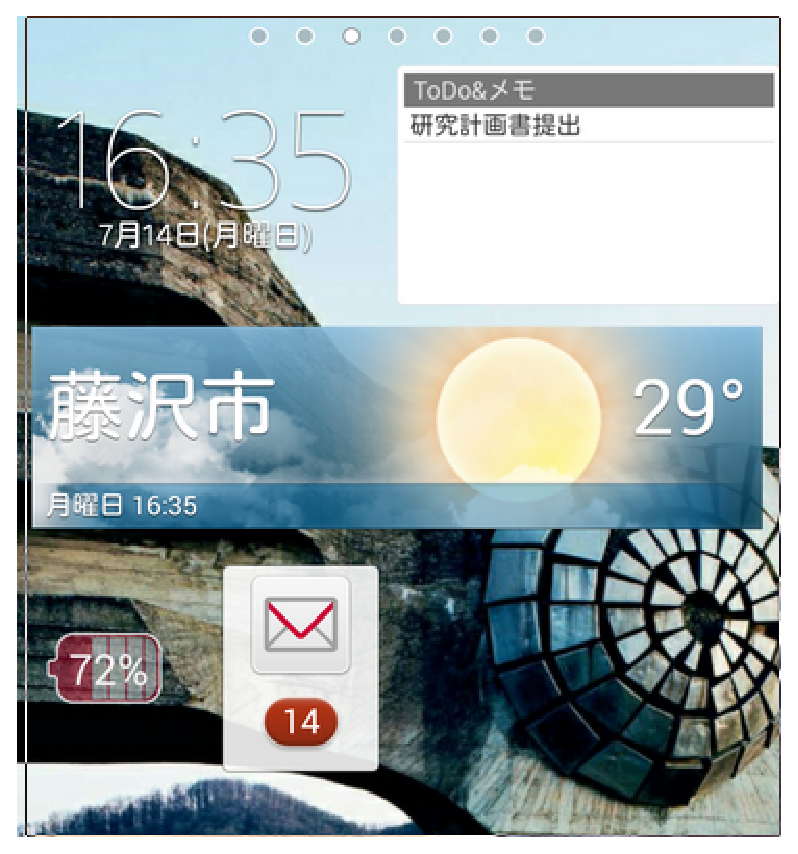
\includegraphics[width=80mm]{image/old_widget.eps}}
    \end{center}
    \caption{現状のWidgetの使用した画面}
    \label{fig:old_widget}
  \end{minipage}
\end{figure}

\section{目的}
あらゆる情報を容易に獲得するための手法を提案・作成する。まずはユーザーが必要とする可能性のある情報を予め取得し、記録しておくことが必要である。次に記録したデータからユーザーが求めるもののみを選択しユーザーに提供することでユーザーが取得したい情報のみをいつでも取得できている状況を作り出す。

\section{本論文の構成}
第\ref{chap:introduction}章では本研究の概要を書いた。

第\ref{chap:contents}章では研究内容を説明する。第\ref{chap:prototype}章ではプロトタイプの実装方法を解説する。第\ref{chap:consideration}章では考察を書く。最後に第\ref{chap:conclusion}章にて結論を書き本論文をしめることとする。添付として参考文献を追記する。
